%% Overleaf			
%% Software Manual and Technical Document Template	
%% 									
%% This provides an example of a software manual created in Overleaf.

\documentclass{ol-softwaremanual}

% Packages used in this example
\usepackage{graphicx}  % for including images
\usepackage{microtype} % for typographical enhancements
\usepackage{minted}    % for code listings
\usepackage{amsmath}   % for equations and mathematics
\usepackage{titlesec}
\usepackage{tikz, blindtext}
\usepackage{mdframed}
\usepackage{listings}
\usepackage{sectsty}
\usepackage{graphicx}
\usepackage{menukeys}
\usepackage{float}

\graphicspath{{pics/}}

\lstset{
    basicstyle        = \small\ttfamily\fontseries{regular}\selectfont,
    columns           = flexible,
    breaklines        = true,
    breakatwhitespace = true % Absolutely counterintuitive
}

\setminted{style=friendly,fontsize=\small}
\usepackage{hyperref}  % for hyperlinks
\usepackage[a4paper,top=4.2cm,bottom=4.2cm,left=3.5cm,right=3.5cm]{geometry} % for setting page size and margins

\definecolor{titlecolor}{rgb}{0.06, 0.25, 0.33}


\sectionfont{\color{titlecolor}}
\subsectionfont{\color{titlecolor}}


\newmdenv[
    topline=false,
    bottomline=false,
    rightline=false,
    linewidth=3pt,
    linecolor=titlecolor,
    innerleftmargin=5pt,
    leftmargin=10pt,
    rightmargin=0pt,
    innerrightmargin=0pt,
]{protip}

\newlength\ChapWd
\settowidth\ChapWd{\huge\chaptertitlename}

\titleformat{\chapter}[display]
  {\normalfont\filleft\sffamily}
  {\tikz[remember picture,overlay]
    {
    \node[fill=titlecolor,font=\fontsize{60}{72}\selectfont\color{white},anchor=north east,minimum size=\ChapWd] 
      at ([xshift=-100pt,yshift=-100pt]current page.north east) 
      (numb) {\thechapter};
    \node[rotate=90,anchor=south,inner sep=0pt,font=\huge,color=gray] at (numb.west) {\chaptertitlename};
    }
  }{0pt}{\fontsize{33}{0}\selectfont\color{titlecolor}}[\rule{\textwidth}{1.5pt}]
\titlespacing*{\chapter}
  {0pt}{50pt}{10pt}


    
% Custom macros used in this example document
\newcommand{\doclink}[2]{\href{#1}{#2}\footnote{\url{#1}}}
\newcommand{\cs}[1]{\texttt{\textbackslash #1}}

% Frontmatter data; appears on title page
\title{SigDigger User's Manual}
\version{0.3.0}
\author{Gonzalo José Carracedo Carballal}
\softwarelogo{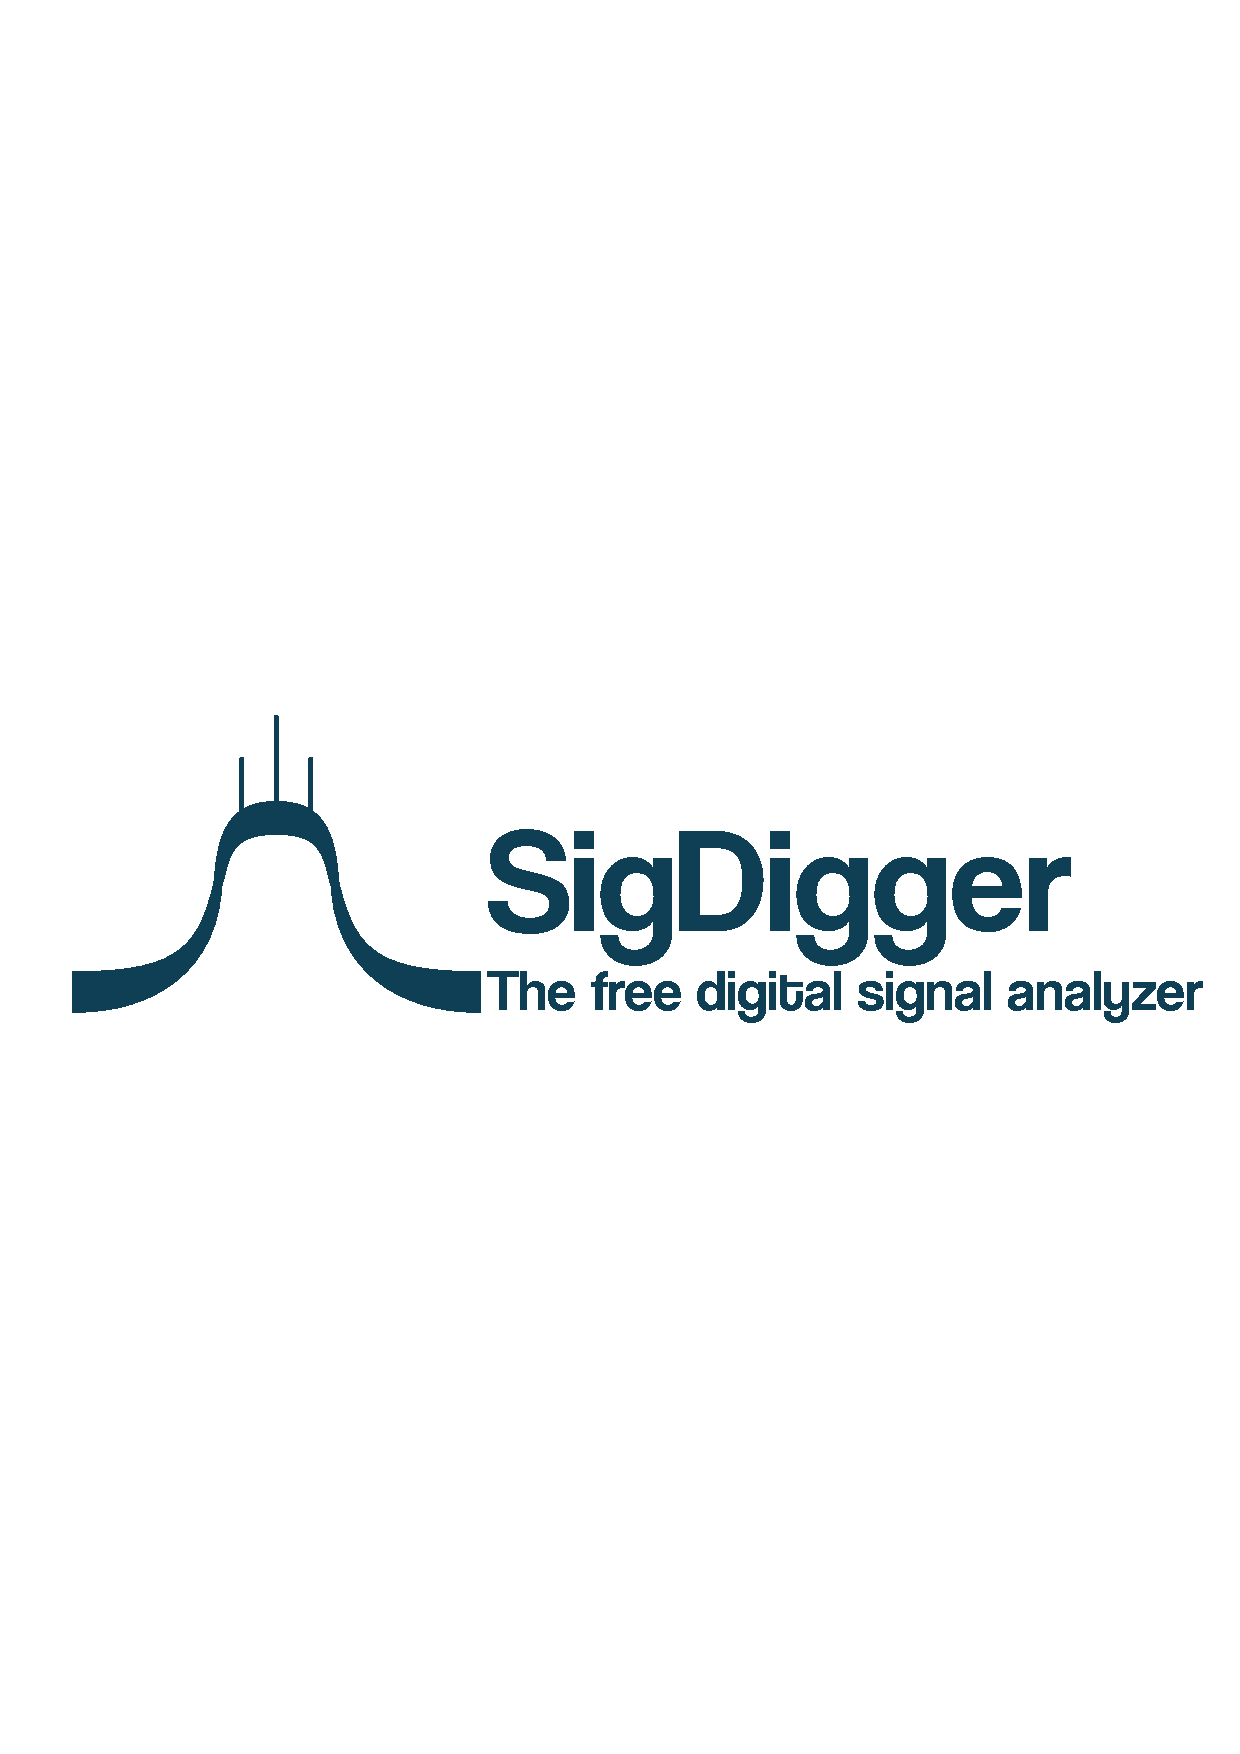
\includegraphics[width=12cm]{logo}}

\begin{document}
\setcounter{secnumdepth}{0}
\maketitle

\tableofcontents

% Required to prevent initial paragraph indentation and placing line breaks between paragraphs.
\setlength{\parindent}{0pt}
\setlength{\parskip}{.5\baselineskip}

\chapter{Introduction}
\fontseries{light}\selectfont
Thank you for choosing SigDigger. The following chapters attempt to cover all the relevant functions from the perspective of a user with minimal knowledge on digital signal processing and radio signals. It also includes practical examples for many real-world applications, including blind demodulation of radio signals and data acquisition from amateur satellites. 

\section{About SigDigger}
SigDigger is a \doclink{https://www.gnu.org/philosophy/free-sw.html}{free} graphical digital signal analyzer. Its main use case is the reverse engineering of radio signals, in which some (or all) parameters of the signal of interest are unknown. This is achieved by a set of features that enable interactive measuring and guessing of the unknown parameters.

SigDigger is compatible with most SDR receivers in the consumer market thanks to the \doclink{https://github.com/pothosware/SoapySDR/wiki}{SoapySDR} support library. It also supports record and playback of RF/IF sample data to and from multiple file formats, including WAV and raw complex float I/Q.

In addition to the reverse engineering-related features, it can be used as a regular spectrum analyzer with multiple visualization functions. It also support real-time audio demodulation of FM, AM and SSB signals.

\section{About the author}
\doclink{https://actinid.org}{Gonzalo José Carracedo Carballal} (BatchDrake) is a software engineer with a background in cybersecurity, mathematical engineering and astrophysics. He has been in love with radio and radioastronomy since he first watched \doclink{https://www.imdb.com/title/tt0118884/}{Contact} circa 1997. He likes coding for fun in his spare time and maintains a number of free software projects in his \doclink{https://github.com/BatchDrake}{public GitHub account}.

\chapter{Installing SigDigger}
SigDigger is designed to work in most Unix-like operating systems. Nonetheless, official support with precompiled binaries is only available for x86-64 based modern GNU/Linux and macOS systems.

Precompiled releases can be downloaded directly from \doclink{https://github.com/BatchDrake/SigDigger/releases}{the GitHub page}. Usually, two types of releases are available:
\begin{itemize}
    \item \textbf{Development builds}, containing the latest features with minimal testing.
    \item \textbf{Stable releases}, with the latest bug-fixes and ready for inclusion in 3rd-party repositories.
\end{itemize}

\section{GNU/Linux}
Precompiled binaries in \doclink{https://appimage.org/}{AppImage} format exist for x86-64 GNU/Linux systems with glibc version 2.27 and newer. AppImage files are self-contained executables and therefore easy to run. Open a terminal, change to the directory in which the AppImage file was downloaded and give execute permissions to it (this is something that needs to be done only once):

\begin{lstlisting}
$ chmod a+x SigDigger-0.3.0-x86_64-full.AppImage
\end{lstlisting}

Now you can execute by typing:

\begin{lstlisting}
$ ./SigDigger-0.3.0-x86_64-full.AppImage
\end{lstlisting}

\begin{protip}
\textbf{Pro Tip:} The AppImage file is a container not only for SigDigger but also for \doclink{https://batchdrake.github.io/suscli/}{suscli and RMSViewer}. Depending on the file name of the AppImage, one of these tools is executed. Some users find handy to have these tools available from the command line by creating symbolic links to them in directories of their \texttt{\$PATH} variable. 
Assuming that \texttt{/usr/local/bin} is in your \texttt{\$PATH} and the AppImage file is in \texttt{\$PWD}, run:

\begin{lstlisting}
$ sudo ln -s $PWD/SigDigger-0.3.0-x86_64-full.AppImage /usr/local/bin/SigDigger
$ sudo ln -s $PWD/SigDigger-0.3.0-x86_64-full.AppImage /usr/local/bin/RMSViewer
$ sudo ln -s $PWD/SigDigger-0.3.0-x86_64-full.AppImage /usr/local/bin/suscli
\end{lstlisting}

This will let you run \texttt{SigDigger}, \texttt{suscli} and \texttt{RMSViewer} from anywhere in the command line.
\end{protip}

\section{macOS}
Precompiled bundles are distributed in \texttt{.dmg} image files for x86-64 processors only. Although there is no official support for M1 processors (yet), x86-64 bundles can still be executed in newer computers by installing \doclink{https://en.wikipedia.org/wiki/Rosetta_(software)}{Rosetta}.

Once you have downloaded the \texttt{.dmg} file, opening SigDigger is straight-forward. Just open the \texttt{.dmg} file and double-click the SigDigger icon to start it.

\begin{protip}
    \textbf{Note:} SigDigger bundles are not currently being signed. You may need to authorize the execution of SigDigger explicitly by \doclink{https://support.apple.com/guide/mac-help/mh40616/mac}{enabling running software from unidentified developers}.
\end{protip}
\section{Microsoft Windows}
There is no official support for Windows, and there are no immediate plans to make it available any time soon. The C99 compiler for Visual Studio does not implement complex arithmetics (which is a fundamental requirement to build SigDigger's core C libraries, namely \texttt{suscan} and \texttt{sigutils}), and I never managed to have a fully automated MinGW-based build system working.

Some users reported being able to build and run SigDigger from WSL/WSL2 with no access to real-world SDR devices. However, the performance of SigDigger under this setup is far from optimal and therefore is not supported either.

This does not mean I am opposed to it, I simply do not have the resources (both software and time) to make it possible. Nonetheless, if you adapted the build system to make it work, \doclink{https://github.com/BatchDrake/SigDigger/pulls}{send me a pull request} and I will be happy to review it.

\section{Building from sources}
SigDigger has been designed to be easily built in Unix-like systems. Nonetheless, the following dependencies are required:

\begin{itemize}
    \item A modern C/C++ compiler (GCC or clang)
    \item Git
    \item CMake (version 3.5.1 or newer)
    \item libsndfile
    \item libfftw3
    \item volk (version 1.0 or newer)
    \item SoapySDR (version 0.5 or newer)
    \item libxml 2.0
    \item PortAudio 2.0
    \item Qt 5 (at least 5.15)
    \item cURL
    \item ALSA libraries (for GNU/Linux targets only)
\end{itemize}

Any mainstream GNU/Linux distribution should maintain packages for these dependencies in their public repositories, under one name or another. In the particular case of \textbf{Debian-based systems} (like Ubuntu), all of these dependencies can be installed with a single command:

\begin{lstlisting}
$ sudo apt install build-essential cmake qtbase5-dev libsndfile1-dev libvolk1-dev libcurl4-openssl-dev libfftw3-dev soapysdr-module-all libsoapysdr-dev libxml2-dev portaudio19-dev libasound2-dev 
\end{lstlisting}

In \textbf{macOS systems} with \texttt{brew}, the procedure is a bit more complicated as it involves installing Qt 5 manually and preparing SoapySDR taps.

The first step is installing --in this order-- Xcode (available from \doclink{https://developer.apple.com/download/}{Apple's developer website}) and Qt 5.15 (\doclink{https://doc.qt.io/qt-5/gettingstarted.html}{tutorial here}).

Once both Xcode and Qt are installed, run the following commands as regular user:

\begin{lstlisting}
$ brew install libsndfile volk curl fftw
$ brew tap pothosware/homebrew-pothos && brew update
$ brew install pothossoapy
$ rm -f /usr/local/lib/libSoapySDR.0.8.dylib
$ brew install soapyrtlsdr soapyhackrf soapybladerf soapyairspy soapyairspyhf soapyredpitaya soapyiris limesuite soapyplutosdr
$ brew install libxml2
$ brew install portaudio
\end{lstlisting}

Once all dependencies have been satisfied, the user can choose one of the following ways to compile SigDigger:

\subsection{Fully-automated build using BLSD (GNU/Linux only)}
BLSD (short for Build Latest SigDigger from Develop) is a shell script that builds SigDigger from development branch and installs it inside a subdirectory of the current working directory.  This is an option for users that do not want to install files in system-wide locations or have no root access to their system. 

The resulting directory (named \texttt{blsd-dir}) contains a folder named \texttt{SigDigger} that can be placed anywhere in the system. Inside the \texttt{SigDigger} folder two executable launcher scripts can be found: \texttt{SigDigger} and \texttt{suscli}. The user may run any of these directly from the command line.

Running BLSD is straight-forward. You can download the script from \doclink{http://actinid.org/blsd}{here}, give execute permissions to it and run it as regular user:

\begin{lstlisting}
$ chmod a+x blsd
$ ./blsd
\end{lstlisting}

Once \texttt{blsd} has finished successfully, navigate to the resulting folder to run SigDigger normally:

\begin{lstlisting}
$ cd blsd-dir/SigDigger
$ ./SigDigger
\end{lstlisting}

\subsection{Manual compilation (all systems)}
This is the option you would choose if you do not have GNU/Linux or want to install SigDigger system-wide. Before building SigDigger, you have to ask yourself which branch do you want to build (\textbf{master} for the latest stable release, \textbf{develop} for the one with the latest features). In order to clone from \textbf{master}, run:

\begin{lstlisting}
$ git clone https://github.com/BatchDrake/sigutils
$ git clone https://github.com/BatchDrake/suscan
$ git clone https://github.com/BatchDrake/SuWidget
$ git clone https://github.com/BatchDrake/SigDigger
\end{lstlisting}

In order to clone from \textbf{develop}, you have to specify the branch explicitly:

\begin{lstlisting}
$ git clone -b develop https://github.com/BatchDrake/sigutils
$ git clone -b develop https://github.com/BatchDrake/suscan
$ git clone -b develop https://github.com/BatchDrake/SuWidget
$ git clone -b develop https://github.com/BatchDrake/SigDigger
\end{lstlisting}

Now, in this order, build and install \texttt{sigutils}:

\begin{lstlisting}
$ cd sigutils
$ mkdir build && cd build
$ cmake ..
$ make
$ sudo make install
$ cd ../..
\end{lstlisting}

Build and install \texttt{suscan}:

\begin{lstlisting}
$ cd suscan
$ mkdir build && cd build
$ cmake ..
$ make
$ sudo make install
$ cd ../..
\end{lstlisting}

Build and install \texttt{SuWidgets}:

\begin{lstlisting}
$ cd SuWidgets
$ qmake SuWidgetsLib.pro
$ make
$ sudo make install
\end{lstlisting}

And finish by building and installing \texttt{SigDigger}:

\begin{lstlisting}
$ cd SigDigger
$ qmake SigDigger.pro
$ make
$ sudo make install
\end{lstlisting}

Now you should be able to execute SigDigger from the command line by typing:

\begin{lstlisting}
$ SigDigger
\end{lstlisting}

\begin{protip}
\textbf{Note:} unless specified, everything will be installed under \texttt{/usr/local}. While this works for many users, you may need to update your environment variables for the previous commands to work:

\begin{lstlisting}
$ export LD_LIBRARY_PATH=/usr/local/lib:"$LD_LIBRARY_PATH"
$ export PKG_CONFIG_PATH=/usr/local/lib/pkgconfig:"$PKG_CONFIG_PATH"
$ export PATH=/usr/local/bin:"$PATH"
\end{lstlisting}

In case you wanted to install SigDigger somewhere else (e.g. \texttt{/usr}), you must pass \texttt{-DCMAKE\_INSTALL\_PREFIX=/usr} command line option to every \texttt{cmake} invocation, \texttt{PREFIX=/usr} to every \texttt{qmake} invocation and an additional \texttt{SUWIDGETS\_PREFIX=/usr} to SigDigger's \texttt{qmake} invocation.
\end{protip}

\chapter{Basic operation}
This chapter covers the features related to signal acquisition, visualization and storage. 
\section{Interface overview}
SigDigger's main window can be divided in 5 areas:
\begin{figure}[!ht]
    \centering
    \includegraphics[width=\textwidth]{mainwindow}
    \caption{Main window}
    \label{fig:mainwindow}
\end{figure}
\begin{enumerate}
    \item \textbf{The spectrum view}, displaying the power spectral density of the signal in real time. The spectrum view also enables the interactive selection of channels by means of an adjustable \textbf{filter box} (shaded green rectangle with a vertical red line). 
    \item \textbf{The waterfall}, displaying a spectrogram of the latest seconds of the signal.
    \item \textbf{The toolbar}, from which one can start/stop the signal capture, configure the application and manage bookmarks.
    \item \textbf{The time slider}, which enables random positioning when the signal is being played back from a capture file (hidden in real-time signal sources)
    \item \textbf{The side bar}, which provides different analysis and visualization functions related to the signal being captured.
\end{enumerate}

The toolbar hosts shortcut buttons to the most frequently used operations. From left to right, these operations are \textbf{Start/Stop capture}, \textbf{Settings}, \textbf{Add bookmark}, \textbf{Manage bookmarks} and \textbf{About SigDigger}.

\begin{figure}[!ht]
    \centering
    \includegraphics[width=.3\textwidth]{toolbar}
    \caption{Toolbar buttons}
    \label{fig:toolbar}
\end{figure}

Other SigDigger functions are directly available from the side bar, grouped in 4 categories: \textbf{Audio preview} (used to play the channel defined by the filter box), \textbf{Signal source} (used to perform different adjustments to the signal source in real time), \textbf{Inspection} (used to inspect the contents of the selected channel in different ways) and \textbf{FFT} (used to adjust different parameters of the spectrum / waterfall view). 

Since the side bar serves as a container for many different controls that cannot fit in a single window, each group can be expanded / collapsed by clicking on its title. Optionally, the side bar can be hidden completely by dragging its left side to the right.

\section{Configuring the signal source}
The first step prior to any signal analysis is telling SigDigger what the signal source will be. This can be done by opening the Settings dialog, either by clicking the corresponding button in the toolbar or by pressing \texttt{Ctrl+S} (\texttt{\cmd+S} in macOS).

The settings dialog consists of several tabs: \textbf{Source}, \textbf{Colors}, \textbf{GUI behavior}, \textbf{TLE Sources} and \textbf{Location}. By default, the Source tab --corresponding to the configuration of the signal source-- is shown. 

Any saved signal source configuration with a name is called a \textbf{profile}. By default, SigDigger uses a profile named \textbf{UI profile} to load and save its signal source configuration. The Source tab is simply an editor of this profile, with additional functions to make copies of it with different names (\texttt{Save as...}) and overwrite it with the contents of existing profiles (\texttt{Load profile}).

\newpage
\begin{figure}[H]
    \centering
    \includegraphics[width=\textwidth]{settings-sdr}
    \label{fig:settings-sdr}
\end{figure}

WIP

\section{Starting a capture}
\section{Real-time source tweaks}
\section{Adjusting the FFT}
\section{Audio preview}
\section{Saving samples}

\chapter{Channel inspection}
TODO
\section{Deferred inspection: the time window}
\subsection{Display controls}
\subsection{Basic measurements}
\subsection{Saving samples}
\subsection{Sampling}

\section{Real-time inspection: inspector tabs}
\subsection{DSP pipeline}
\subsection{Interface overview}
\subsection{Spectrum sources}
\subsection{Fine-tuning}
\subsection{Parameter estimation}
\subsection{Demodulator control}
\subsection{Data forwarding}

\chapter{Panoramic spectrum}
TODO
\section{Interface overview}
\section{Strategy and partitioning}
\section{Saving data}

\chapter{Advanced features}
TODO
\section{Doppler corrections}
\section{Subcarrier inspection}
\section{Analog TV}
\section{Remote analyzers}

\appendix

\chapter{Example use cases}
TODO
\section{Blind demodulation of a BPSK signal}
\section{Blind demodulation of a GMSK signal}
\section{Demodulation of the RDS signal of a FM station}
\section{Demodulation of a space probe downlink}
\section{Blind demodulation of a WeFax signal}
\section{APT decoding}

\chapter{Device-specific tweaks}
TODO
\section{RTL-SDR}
\subsection{Bias tee}
\subsection{Direct sampling}
\section{HackRF}
\subsection{Bias tee}

\end{document}
